\documentclass[12pt]{article}

\usepackage[utf8]{inputenc}
\usepackage[margin=1in]{geometry}
\usepackage[titletoc,title]{appendix}
\usepackage[section]{placeins}  % allows us to stop floaters
\usepackage{longtable}  % for bringing in our data tables to the appendix
\usepackage{amsmath,amsfonts,amssymb,mathtools}
\usepackage{graphicx,float}
\usepackage{makecell}
\usepackage{caption}
\usepackage{csvsimple,booktabs} % load csv data into table
\usepackage{filecontents} % read csv data contents
\usepackage{indentfirst} % set first paragraph of each section to be indented
\usepackage[backend=biber,style=authoryear]{biblatex} % style our references

\addbibresource{references.bib} % load resources from bib file
\setlength{\parindent}{1.5em} % set indent length for each paragraph
\graphicspath{ {../figures/} }

\newcommand*\mean[1]{\overline{#1}}

\title{EOSC 453 Assignment 2\\
\large Volcanic Eruptions and Climate Change}
\author{
    E. Giroud-Proeschel - 123456789 \\
    P. Matlashewski - 45701109\\
    M. Ormerod - 16265167
}

\begin{document}

\maketitle
\newpage
\tableofcontents
\newpage

% Introduction and Overview
\section{Introduction}
Anthropogenic global warming is an identifier of climate change and has
manifested as a defining issue of our time; intensifying the frequency and
severity of extreme weather events, producing sea-level rise with the potential
to displace millions, causing the loss of large freshwater reservoirs, reducing
biodiversity in key biomes, among other effects. Though the question of why, and
how, climate change operates, and what we can do to mitigate its effect on the
Earth of our lifetime, is an arduously nonlinear problem that climate scientists
have battled with for decades, both in the laboratory and in politics. One of
the questions within this contention is how large local out-gassing events of
volatile aerosols during volcanic eruptions, like carbon dioxide and sulfur
dioxide, have historically affected the Earth, from the last ice-age to the
explosive evolution following it. Here we have developed a simple radiative
energy balance model for the Earth in order to investigate the effects of
volcanism on this energy balance's behaviour. This model is inspired by the
work of Russian climatologist Mikhail I. Budyko of the Lenningrad Geophysics
Observatory, who discovered the ice-albedo feedback mechanism underlying climate
change through his pioneering of studies on global climate using physical models
of equilibrium (\cite{budyko_albedo}).

In this report, we will investigate perturbations to our climate model via
volcanic forcing. This will take three forms. We will begin with a presently
undisturbed model that approaches steady-state. Then we analyze the effects of
an added perturbation of volcanic aerosols derived from data collected from the
1982 El Chichón and Pinatubo eruptions published in \cite{robock}. Finally, we
will implement a parameterization of temperature-dependent albedo in conjunction
with a Poisson distribution of volcanic eruptions, temporally and spatially, to
simulate a snowball Earth scenario.
WE SHOULD ADD A BIT ABOUT OUR GENERAL ASSUMPTIONS HERE

\subsection{Budyko Climate Model}

\subsection{Volcanic Eruptions}

\subsubsection{Direct Radiation Occlusion}
\begin{figure}[H]
    \centering
    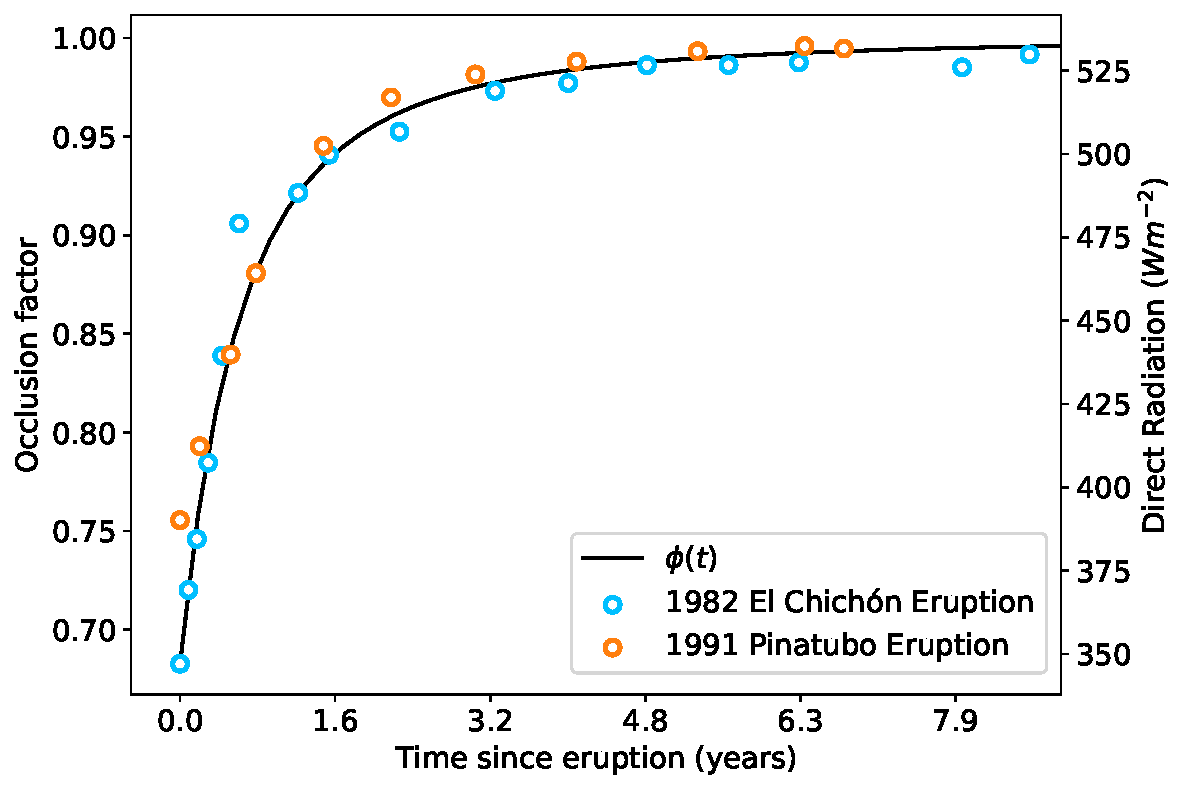
\includegraphics[scale=0.6]{occlusion.pdf}
    \caption{
        Plot of $\phi(t)$; occlusion factor. An occlusion factor of 0.7
        represents a $30\%$ reduction in total incoming solar radiation.
    }
    \label{fig:occlusion}
\end{figure}
\FloatBarrier

\subsubsection{Spatial Distribution of Aerosols}
\begin{figure}[H]
    \centering
    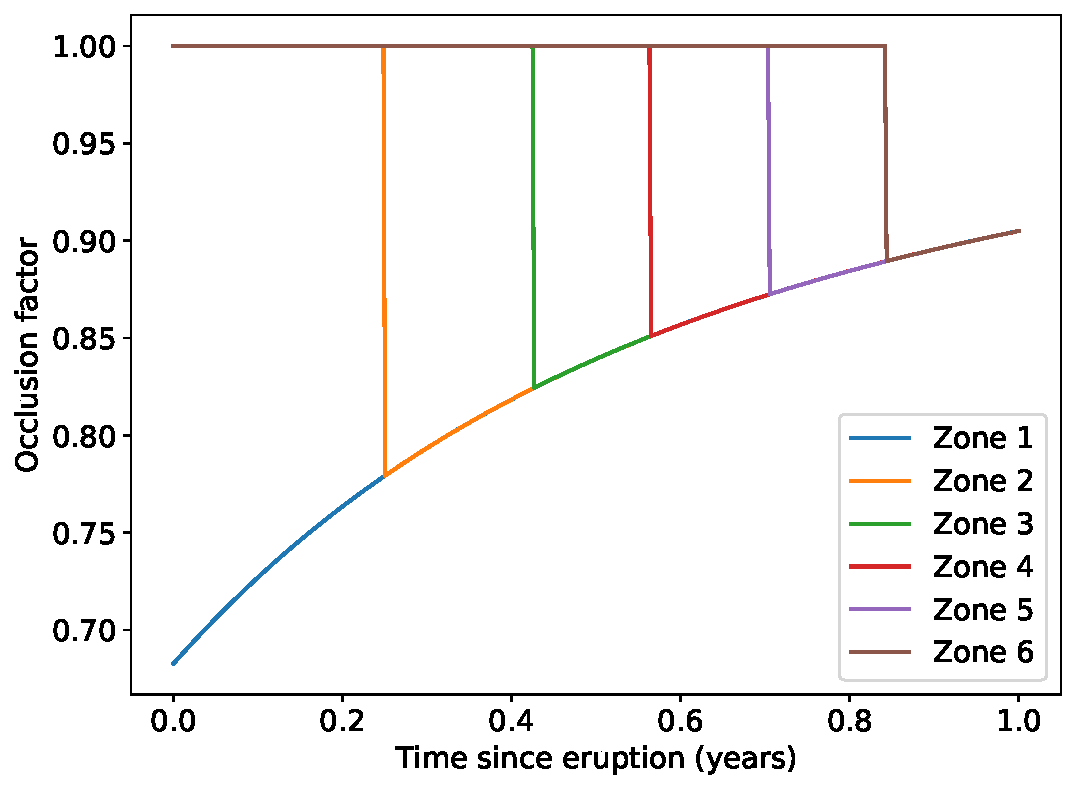
\includegraphics[scale=0.6]{occlusion_space.pdf}
    \caption{
        The spatial effect of eruptions.
    }
    \label{fig:occlusion_space}
\end{figure}
\FloatBarrier

\subsubsection{Stochastic Eruption Frequency}

\subsection{Ice-Albedo Feedback}

\begin{figure}[H]
    \centering
    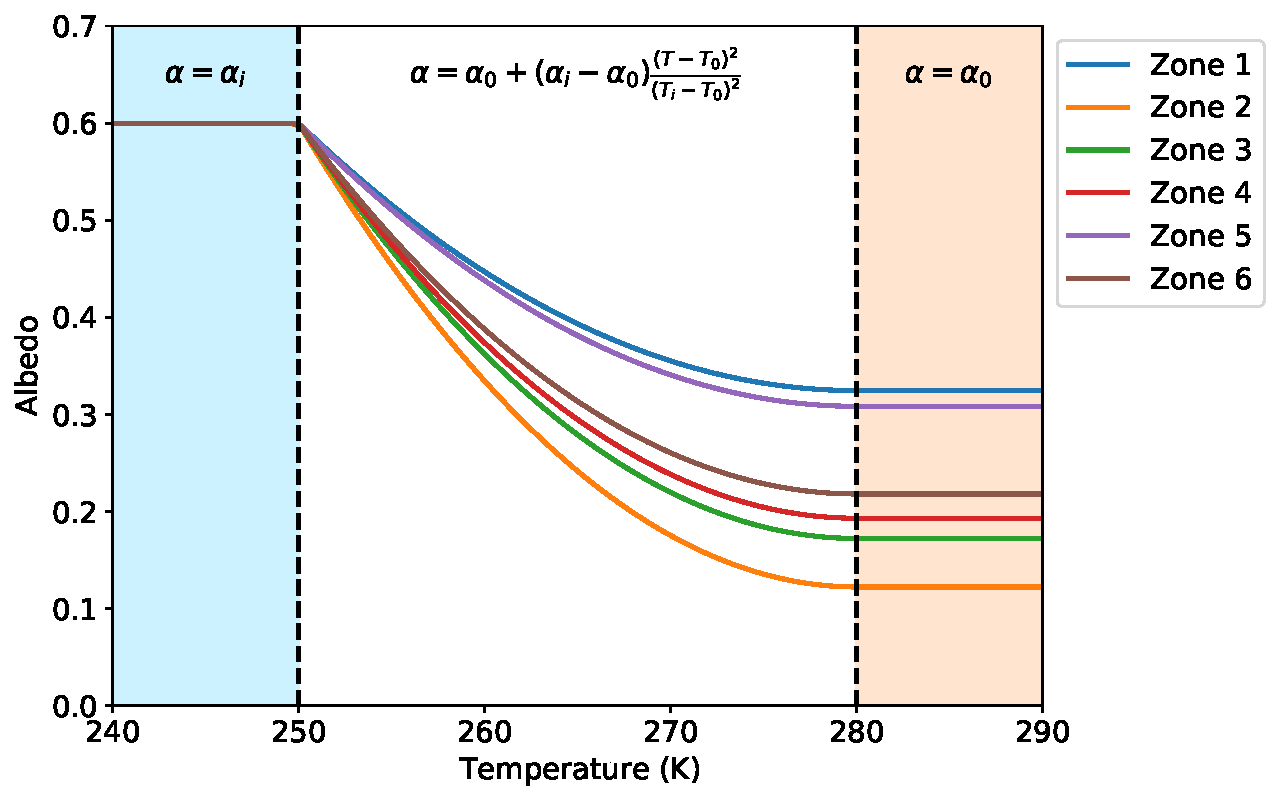
\includegraphics[scale=0.6]{albedo.pdf}
    \caption{
        Albedo parameterization as a function of temperature in each zone.
    }
    \label{fig:albedotemp}
\end{figure}
\FloatBarrier

% Figure results
\section{Results}
\label{section:results}
In this section, we will report on data obtained via our three forms of volcanic
perturbations and describe the behaviours of these perturbations within the
context of the data itself.

\subsection{Steady-State Climate Model: No Volcanism}
By passing initial condition temperatures calculated through our model with
suppressed inter-zonal transfer (See Table \ref{tab:supressedteq}) to our
steady-state model where inter-zonal transfer is allowed, we solve for the
equilibrium temperatures by integrating forward in time
(Figure \ref{fig:steadystate}).

\begin{figure}[H]
    \centering
    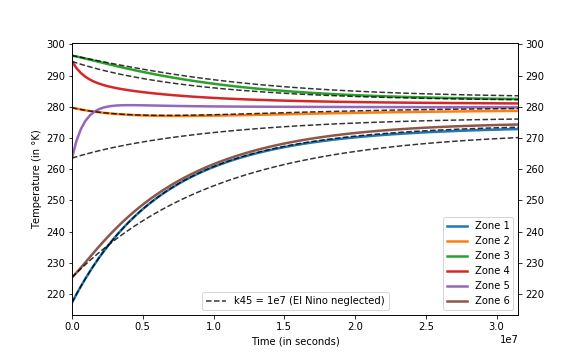
\includegraphics[scale=0.5]{Question2.png}
    \caption{
        Equilibrium solution for 6-zoned Earth climate model. Zone 1 marks the
        southernmost band at $60-90^{\circ}$S while zone 6 represents the
        northernmost band at $60-90^{\circ}$N. Zones 2-5 are bands covering
        $30^{\circ}$ intervals between zones 1 and 6
        (See Figure \ref{fig:zones}).
    }
    \label{fig:steadystate}
\end{figure}
\FloatBarrier

There are a few key observations to note. The first is that a larger transfer
coefficient (\ref{tab:boundaryparams}), representing the northern Gulf Stream
between zones 4 and 5, produces a large initial temperature gradient in these
zones relative to the others (solid colour lines in Figure
\ref{fig:steadystate}). The second is that the highest temperature zones at
equilibrium are 3 and 4, and the lowest temperature zones at equilibrium are 6
and 1. All zones approach an equilibrium temperature between $274.1^{\circ}$K
and $282.3^{\circ}$K after a model year (Table \ref{tab:teq}). By reducing the
inter-zonal transfer coefficient between zones 4 and 5
(dashed lines in Figure \ref{fig:steadystate}), we can alter the characteristics
of a few zones dramatically. The most obvious of which are zones 4, 5, and,
perhaps surprisingly, zone 6. These alterations include a reduction in the
initial rate of change in temperature and will be analyzed further in Section
\ref{section:steadystate}.

\subsection{Climate Model Following Single Volcanic Eruption}
To introduce the effect of volcanism to our model, we add an occlusion factor,
$\phi(t)$, to each zone that reduces total incoming solar radiation
(Figure \ref{fig:occlusion}). $\phi_k(t)$ varies in initial magnitude and onset
time based on proximity to the zone in which the eruption occurs. Alternatively,
an eruption in zone 3 will have a reduced effect in zone 4 and 2 to simulate
the thinning of aerosol density as the cloud spreads, and the aerosols have a
travel time before the effect is felt in adjacent zones. $\phi(t)$ follows a
$\frac{1}{t^2}$ fit to eruption data from \cite{robock} such that
$\lim_{t\to\infty}\phi(t) = 1$.
Figure \ref{fig:oneerupt} shows our solution post eruption. 

Figure \ref{fig:oneerupt} shows the effect of a single eruption on zonal 
temperatures initially at steady-state. The eruption occurs in zone 4 a year into
modelling, as indicated by the colour and position of the vertical dashed line. 
Here, the most important feature is the time lag between zones. Zone 4 is immediately 
affected by the solar occlusion. The subsequently affected zones are 5 and 3, followed 
by 6 and 2, and finally, zone 1. In addition, the initial magnitudes of occlusion 
at each of these zones decreases the further they are, spatially, from the 
initial eruption zone following Figure \ref{fig:occlusion_space}
(i.e $\phi_{4,init} > \phi_{3,5,init} > \phi_{2,6,init} > \phi_{1,init}$).
Finally, recovery by each zone to equilibrium temperatures occurs approximately 
a decade after eruption, to the same relative temperature range as initial, 
steady-state conditions.

\begin{figure}[H]
    \centering
    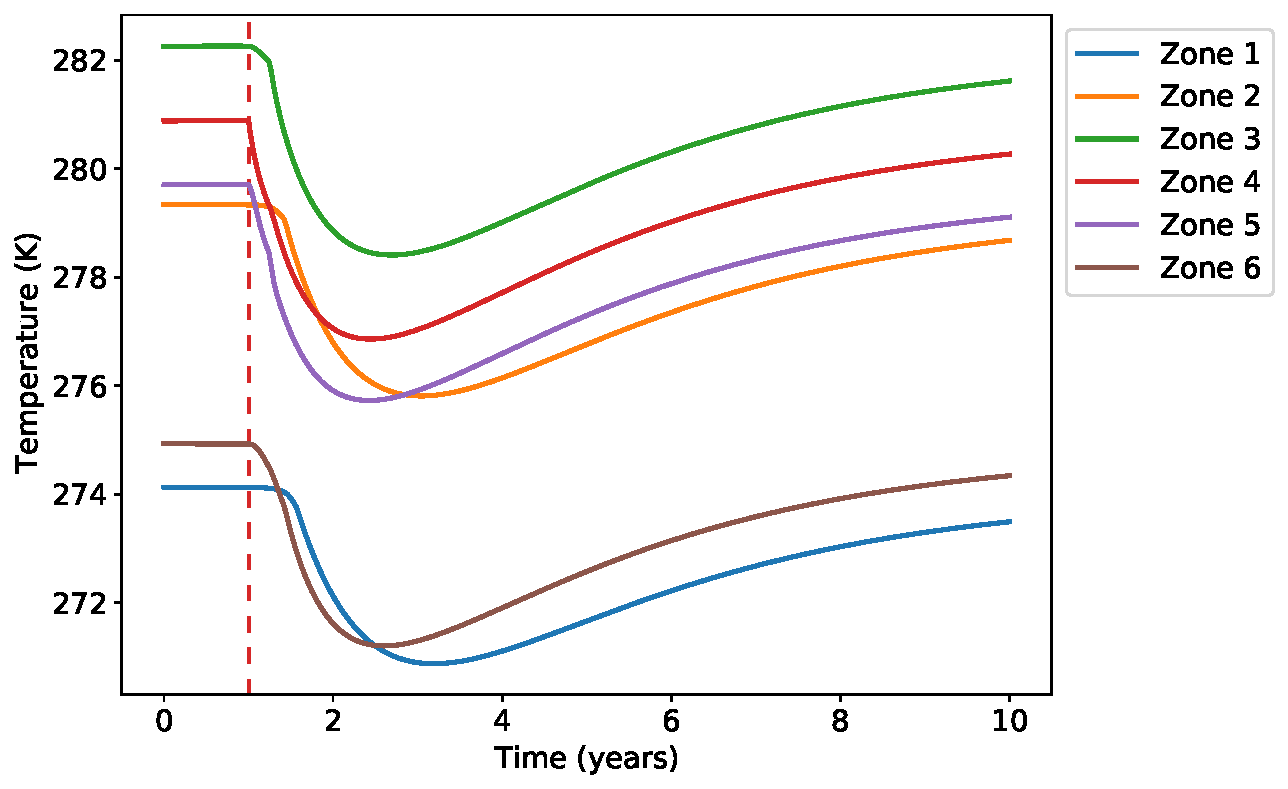
\includegraphics[scale=0.6]{one_eruption.pdf}
    \caption{
        Reduction in solar forcing post eruption results in temperature drop.
    }
    \label{fig:oneerupt}
\end{figure}
\FloatBarrier

\subsection{The Ice-Albedo Effect}
In Figure \ref{fig:albedo_equil} we have coupled our ice albedo parameterization
to our climate model to visualize its dynamic, nonlinear effect on climate forcing.
Hence, we recognize three equilibria, two of which are stable and one that is 
unstable. If we begin the model at the unstable equilibrium temperatures defined 
in Table \ref{tab:eqstates}, a small positive temperature perturbation causes zonal
temperatures to increase asymptotically to the upper equilibrium (dashed lines). 
Conversely, a small negative perturbation causes zonal temperatures to approach the lower 
equilibrium aspymptotically (dotted lines). These scenarios are represented by the 
warm Earth and snowball Earth sections, respectively. Note that the warm Earth 
equilibrium has zonal temperatures that are similar to the steady-state described in
Figure \ref{fig:steadystate}, though zones below the upper threshold temperature 
have temperatures that are slightly perturbed from our original model. In the 
lower equilibrium case, the temperature difference between high-latitudinal and 
mid-latitudinal zones is much smaller.

\begin{center}
    \begin{tabular}{ c | c | c | c }
      \hline
      \thead{Zone} & 
      \thead{Warm Earth \\ Equilibrium Temperature [K]} &
      \thead{Unstable \\ Equilibrium Temperature [K]} &
      \thead{Snowball Earth \\ Equilibrium Temperature [K]} \\
      \hline
        1 & 217.23 & 217.23 & 217.23 \\
        2 & 279.74 & 279.74 & 279.74 \\
        3 & 296.45 & 296.45 & 296.45 \\
        4 & 294.56 & 294.56 & 294.56 \\ 
        5 & 263.56 & 263.56 & 263.56 \\
        6 & 225.33 & 225.33 & 225.33 \\
    \hline
    \label{tab:eqstates}
    \end{tabular}
  \end{center}

% \begin{table}[H]
%     \parbox{.45\linewidth}{
%     \captionsetup{singlelinecheck = false, justification=justified}
%     \caption{Ice-Albedo Temperature Equilibria}
%     \begin{tabular}{ll}
%     \hline
%     \thead{Zone} & \thead{Warm Earth \\ Equilibrium Temperature [$^{\circ}$K]}  \\
%     \hline
%     1 & 217.23 \\
%     2 & 279.74 \\
%     3 & 296.45 \\
%     4 & 294.56 \\ 
%     5 & 263.56 \\
%     6 & 225.33 \\
%     \end{tabular}
%     \label{tab:supressedteq}
% }


\begin{figure}[H]
    \centering
    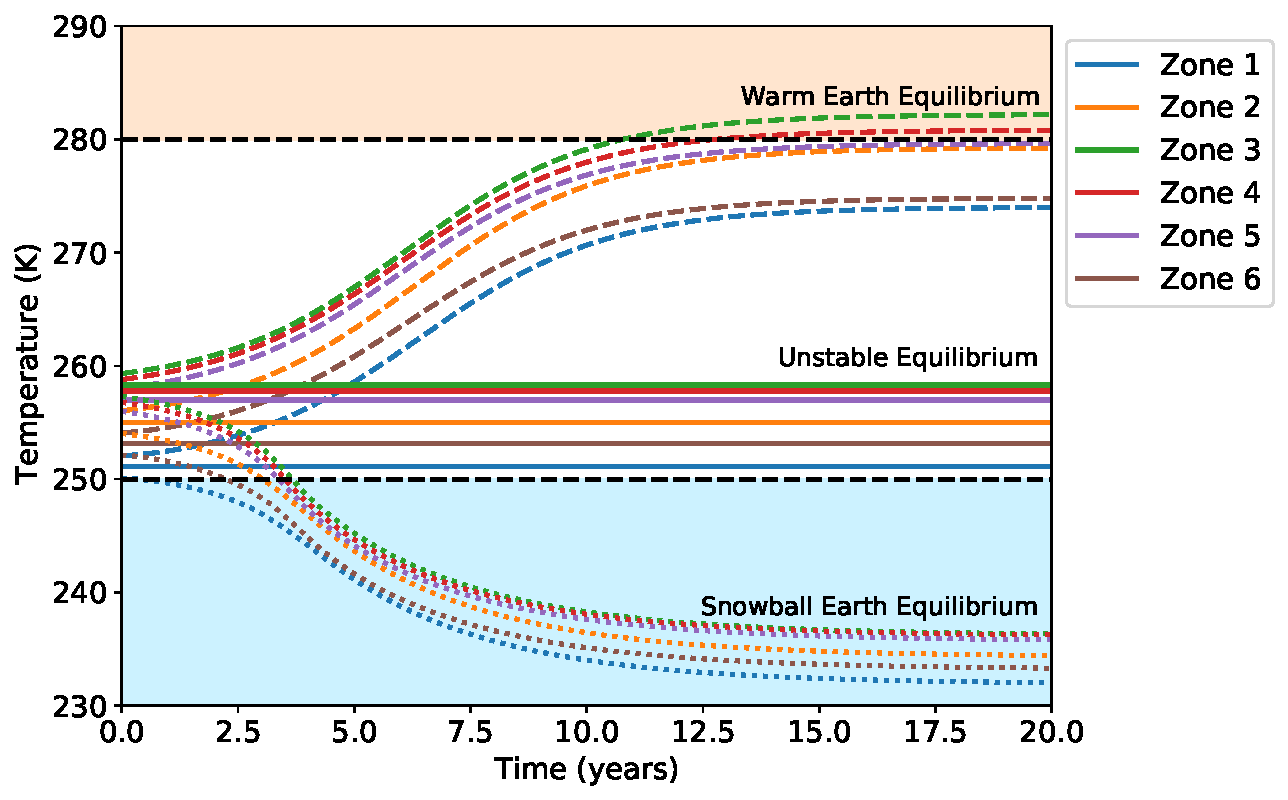
\includegraphics[scale=0.6]{albedo_equilibria_1plot.pdf}
    \caption{
        Integrating through climate model incorporating both stochastic volcanic
        eruptions and ice-albedo feedback parameterization.
    }
    \label{fig:albedo_equil}
\end{figure}
\FloatBarrier

\subsection{Snowball Earth: Stochastic Volcanism and Temperature-Dependent
Albedo} 
As a possible scenario for global glaciation, we couple a Poisson
distribution of eruptions, both temporally and spatially, with a
temperature-dependent parameterization of albedo. This coupling is shown in
Figure \ref{fig:fireandice}, and will be discussed after looking at the
mechanisms in isolation. \\

The interval post-origin for stochastic eruptive behaviour has been extended to
100 years visualize a return to equilibrium more clearly. From Figure
\ref{fig:stocherupt}, we see that following each eruption is a decline in zonal
temperatures, and sufficiently close eruptions, in time, compound that effect.
The distribution lag associated with aerosol spreading is still represented
numerically, though a lag of a few months is difficult to discern visually on
this extended time scale. 

\begin{figure}[H]
    \centering
    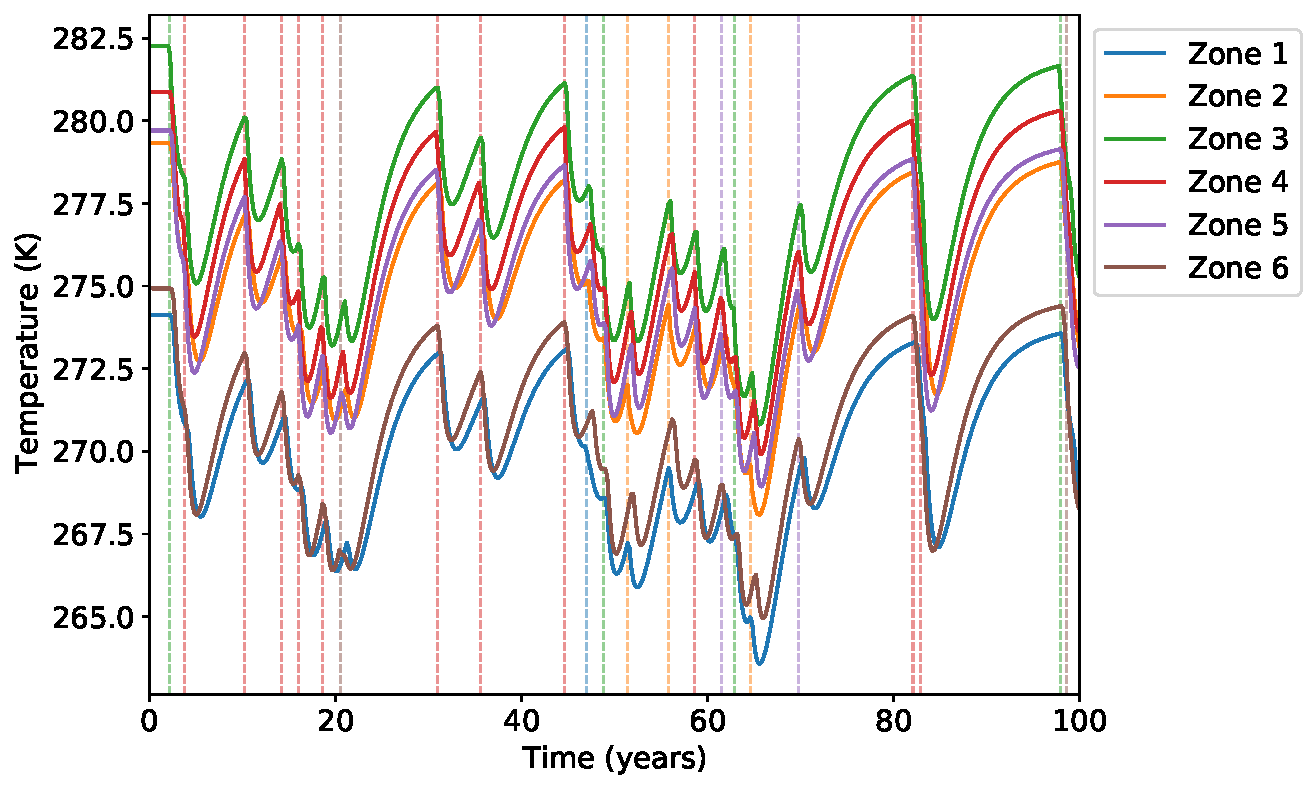
\includegraphics[scale=0.6]{stochastic_eruptions.pdf}
    \caption{
        Stochastic eruption distribution following Poisson distribution.
        Vertical dotted lines are colored based on the zone the eruption
        occurred in, and their placement is the point in time at which the
        eruption is initiated.
    }
    \label{fig:stocherupt}
\end{figure}
\FloatBarrier

\begin{figure}[H]
    \centering
    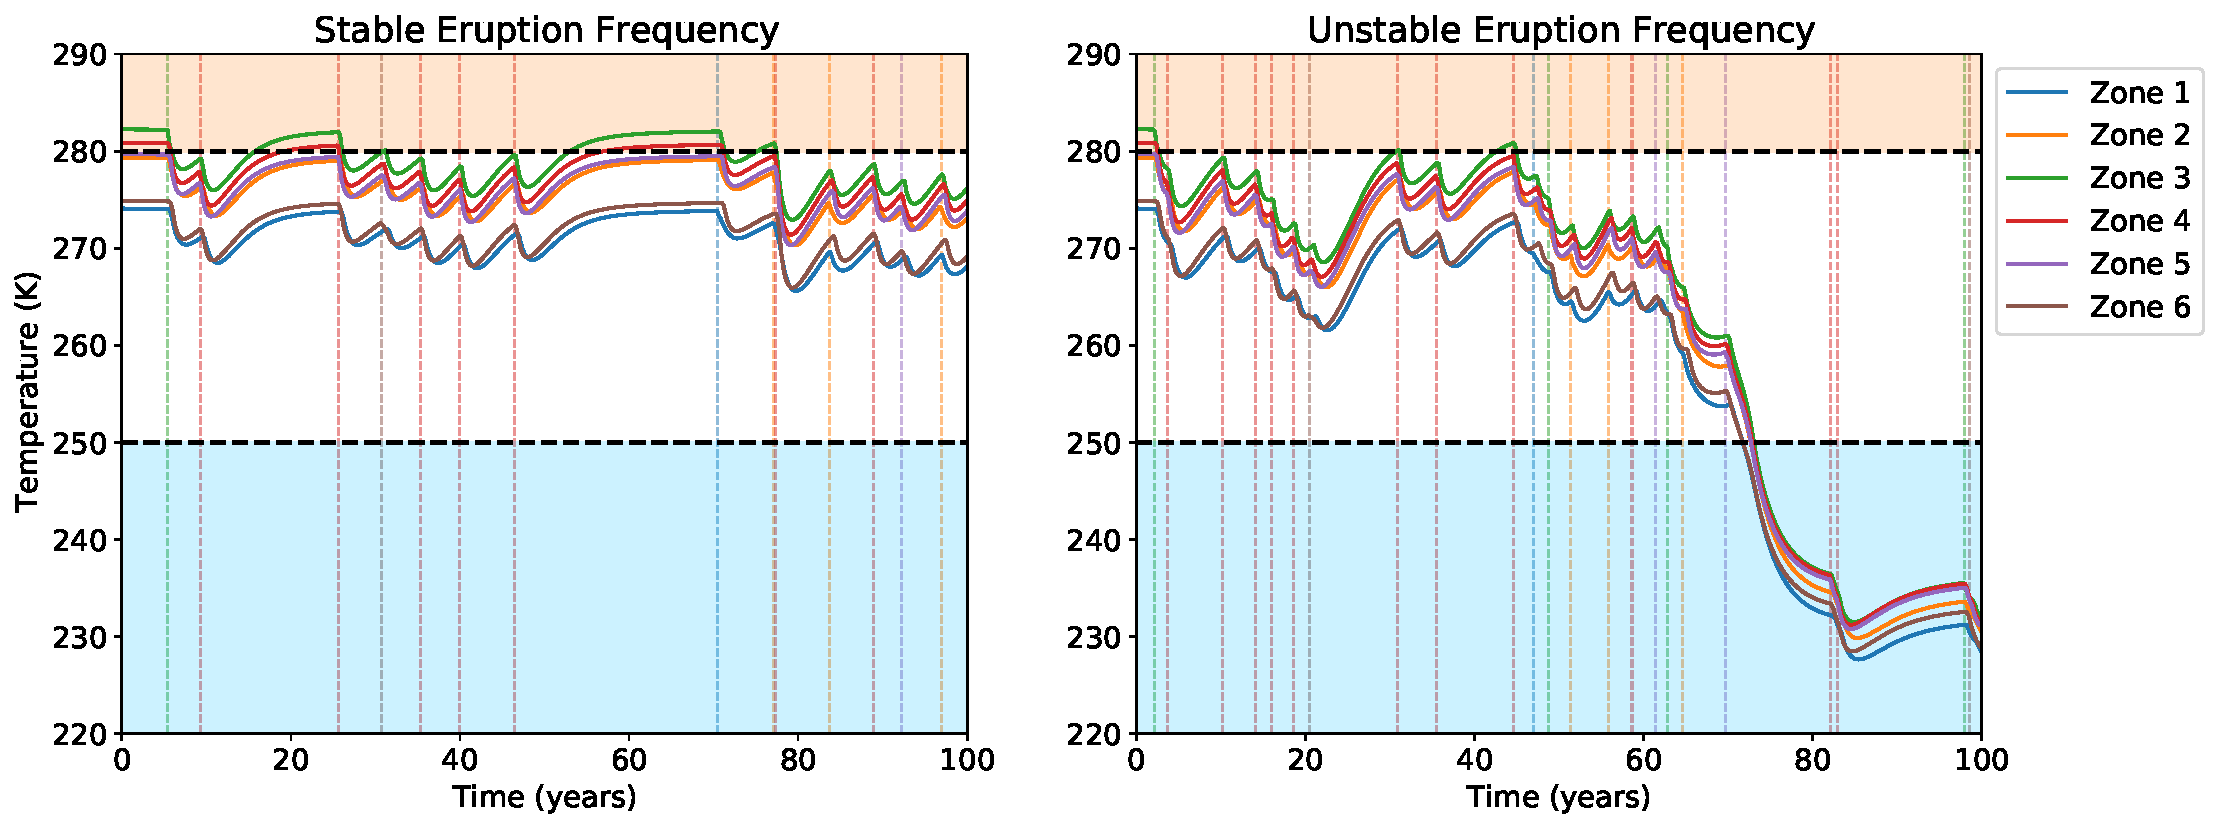
\includegraphics[width=\linewidth]{eruptions_albedo.pdf}
    \caption{
        Integrating through climate model incorporating both stochastic volcanic
        eruptions and ice-albedo feedback parameterization.
    }
    \label{fig:fireandice}
\end{figure}
\FloatBarrier

To incorporate variable albedo, we define a piece-wise albedo parameterization
dependent on zonal temperature (Adapted from \cite{jellinek_ps}).
The parameterization follows the form of Equation\ref{eqn:albedoparam}
(Section \ref{sec:eqns}), and ascribes behavior based on each zone's basal
albedo and temperature range (Figure \ref{fig:albedotemp}). Temperatures above
$280^{\circ}K$ allow each zone to take on their originally defined albedo,
$\alpha_k$ (See Table \ref{tab:zoneparams}). Temperatures below $250^{\circ}K$
replace these with a constant ice albedo, while the interval between describes a
quadratic growth from $\alpha_k$ to $\alpha_i$ as temperature declines.

By coupling these processes, and ranging through a series of initial temperature
conditions in each zone, we are able to find a numerical snowball Earth in
Figure \ref{fig:fireandice}. Similarly to our observations of Figure
\ref{fig:stocherupt}, eruptions that happen close in time have a compounded
effect of driving temperatures down further. After several eruptions between
$1.75e9-2.1e9$ seconds, this effect causes temperatures to drop below the lower
threshold of our albedo parameterization, $T_i$ and plummet to a new state
between approximately $225-245^{\circ}K$. This phenomenon will be expanded on
in Section \ref{sec:snowballearth}.

\section{Discussion}
Here we will discuss the possible processes behind the numerical behavior of our
Figures in Section \ref{section:results} in order to elucidate the connection
between our mathematical and computational results with their underlying
physics.

\subsection{Steady-State Climate Model: No Volcanism}
\label{section:steadystate}
Zones 4 and 5 experience a large initial temperature gradient due to a heat
transfer coefficient indicative of Gulf Stream circulation processes that is
larger than the transfer coefficients between other zones
(Figure \ref{fig:steadystate}). This causes zones 4 and 5 to approach their
equilibrium values more quickly. For example, zone 5 reaches its approximate
equilibrium temperature within the first two months of the model year because
the efficiency of heat transfer between these zones is greater than between
others. \\

Zones 3 and 4 are the warmest zones due to their proximity to Earth's equator.
Both lie within $30^{\circ}$N/S of the equator, and hence have the largest
effective surface area, coupled with a low albedo due to a high land and sea
fraction versus ice fraction (See Table \ref{tab:zoneparams}). This increases
these zones' retention of incoming solar radiative heating by reducing the
amount lost to space as out-going, long-wave radiation (OLR). Zone 3 may be
hotter than zone 4 due to smaller transfer coefficients between its adjacent
zones than compared with zone 4, where heat transfer occurs rapidly due to
influence from the Gulf Stream across the boundary of zone 4 and 5. \\

Conversely, zones 1 and 6 are the coldest zones at equilibrium due to their
placement at Earth's high latitudes ($>60^{\circ}$N/S). This reduces their
effective surface area such that less total solar insolation occurs, alongside
a higher albedo due to a dominating ice fraction. This causes the OLR to be
larger relative to incoming radiative heating than in the case of the other
zones. Hence, temperature at equilibrium in zones 1 and 6 is lower. Zone 1 may
be colder than zone 6 due to a higher albedo associated with a marginally larger
ice fraction that increases OLR even relative to zone 6. \\

Comparing the solid and dashed lines in Figure \ref{fig:steadystate}, there is a
general trend of reduced rate of change in temperature for several northern 
latitudinal zones. Zones 4 and 5 experience the greatest deviation from the
original approach to equilibrium as this change is at their boundary of
separation and directly reduces the amount of heat exchange between them.
Zone 6 also experiences a reduction in the rate of approach to equilibrium due
to its nonlinear relation with zone 5. As we can see, these effects are
compounded in zones closest to zones 4 and 5, such that at sufficient
separation, approaches to equilibrium are not noticeably affected. This is
evident in zones 2 and 1, and suggests they have little dependence on
temperature characteristics within the northern zones. 

\subsection{Climate Model Following Single Volcanic Eruption}
\subsection{The Ice-Albedo Effect}
\subsection{Snowball Earth: Stochastic Volcanism and Temperature-Dependent Albedo}
\label{sec:snowballearth}

\section{Conclusion}
\subsection{Future Work}

\section{Ancillary Information}
\subsection{Author Contributions}

\begin{table}[H]
    \centering
    \begin{tabular}{rrr}
    Section & Subsection & Contributors \\
    \hline
    Graphic & Box-Model & M  \\
    Code & Steady-State Climate & P and E \\
    Code & Perturbation: Single Volcanic Eruption & P, E, and M \\
    Code & Snowball Earth & P, E, and M \\
    Introduction &  & M \\
    Results & Steady-State Climate & n/a \\
    Results & Perturbation: Single Volcanic Eruption & n/a \\
    Results & Snowball Earth & n/a\\
    Discussion & Steady-State Climate Model & n/a \\
    Discussion & Perturbation: Single Volcanic Eruption & n/a \\
    Discussion & Snowball Earth & n/a\\
    Conclusion & Future Work & n/a \\
    Conclusion & Summary & n/a \\
    \end{tabular}
    \caption{
        In descending order: names depict relative contribution to
        sections with more than one contributor.
    }
    \label{tab:contributions}
\end{table}

\subsection{Algorithm Development}
\begin{figure}[H]
    \centering
    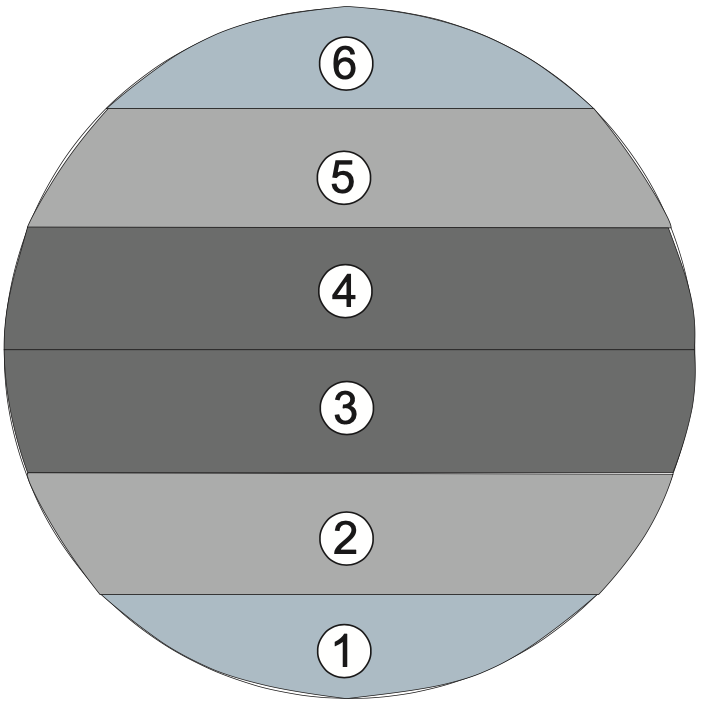
\includegraphics[scale=0.3]{zones.png}
    \caption{Graphic depicting zone intervals.}
    \label{fig:zones}
\end{figure}
\FloatBarrier

\begin{figure}[H]
    \centering
    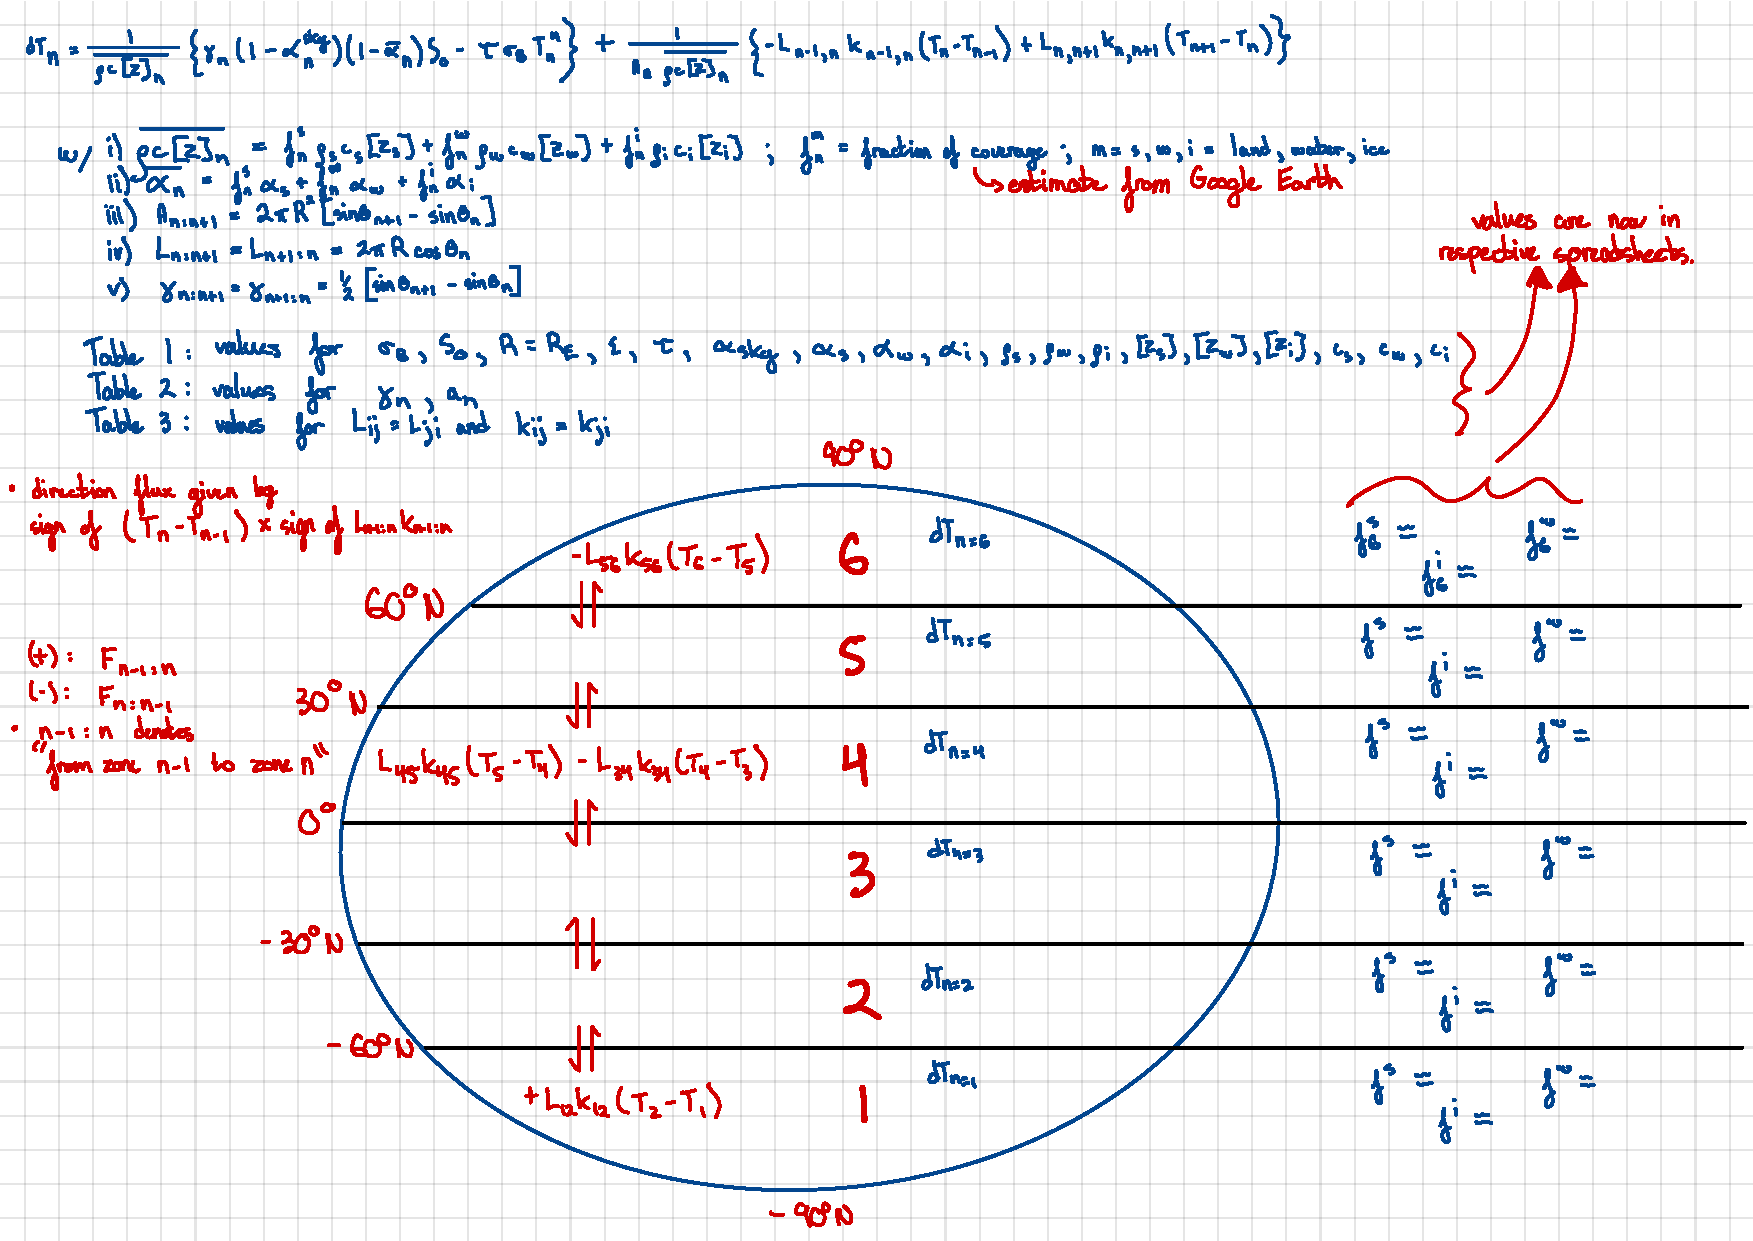
\includegraphics[scale=0.3]{Graphicalg.pdf}
    \caption{
        Sketch depicting zone intervals and necessary parameters for numerical
        solving.
    }
    \label{fig:graphicalg}
\end{figure}
\FloatBarrier

\begin{enumerate}
    \item Identify 6 latitudinal zones. Namely between $0-30^{\circ}NS$,
    $30-60^{\circ}NS$ and $60-90^{\circ}NS$.
    \item Determine parameters associated with each area.
    \item Solve ODE numerically using Paul Matlashewski's
    ClimateModel.py library.  
\end{enumerate}

% \subsection{Python Functions}
% Add your important MATLAB functions here with a brief implementation explanation. This is how to make an \textbf{unordered} list:
% % \begin{itemize}
% %     \item \texttt{y = linspace(x1,x2,n)} returns a row vector of \texttt{n} evenly spaced points between \texttt{x1} and \texttt{x2}. 
% %     \item \texttt{[X,Y] = meshgrid(x,y)} returns 2-D grid coordinates based on the coordinates contained in the vectors \texttt{x} and \texttt{y}. \text{X} is a matrix where each row is a copy of \texttt{x}, and \texttt{Y} is a matrix where each column is a copy of \texttt{y}. The grid represented by the coordinates \texttt{X} and \texttt{Y} has \texttt{length(y)} rows and \texttt{length(x)} columns.  
% % \end{itemize}

% % Python Codes
% \subsection{Python Code}
% Add your Python code here. This section will not be included in your page limit of six pages.
% \begin{listing}[h]
% \inputminted{matlab}{example.m}
% \caption{Example code from external file.}
% \label{listing:examplecode}
% \end{listing}
\subsection{Data}
\subsubsection{Model Equations}
\label{sec:eqns}
\begin{equation} \label{eqn:dtk}
  \frac{dT_k}{dt} = \frac{1}{\mean{\rho_kc_k[Z_k]}}
  \{
    \gamma_k(1-\alpha_k^{sky})(1-\Bar{\alpha_k})S_0-\tau\sigma_BT_k^{4}
  \} +
  \frac{L_{ki}k_{ki}}{{A_k}\mean{\rho_kc_k[Z_k]}}(T_{k}-T_{i}) \quad k=1,\dots,6
\end{equation}

\begin{equation} \label{eqn:dtkphi}
  \frac{dT_k}{dt} = \frac{1}{\mean{\rho_kc_k[Z_k]}}
  \{
    \gamma_k(1-\alpha_k^{sky})(1-\Bar{\alpha_k})\phi_k(t)S_0-\tau\sigma_BT_k^{4}
  \} +
  \frac{L_{ki}k_{ki}}{{A_k}\mean{\rho_kc_k[Z_k]}}(T_{k}-T_{i})
  \quad i \neq k, i = k \pm 1
\end{equation}

\begin{equation} \label{eqn:albedoparam}
  \alpha_k(T_k) =
    \begin{cases}
    \alpha_k & T_k \geq T_0 \\
    \alpha_k + (\alpha_i-\alpha_k)\frac{(T_k-T_0)^2}{(T_i-T_0)^2}
    & T_i < T_k < T_0 \\
    \alpha_i & T_k \leq T_i
    \end{cases}
    \quad T_i = 250^{\circ}K \quad T_0 = 280^{\circ}K
\end{equation}

\subsubsection{Equilibrium Temperatures: Steady State Model}
\begin{table}[H]
    \parbox{.45\linewidth}{
    \captionsetup{singlelinecheck = false, justification=justified}
    \caption{Inter-zonal heat transfer suppressed}
    \begin{tabular}{ll}
    \hline
    Zone & Equilibrium Temperature [$^{\circ}$K] \\
    \hline
    1 & 217.23 \\
    2 & 279.74 \\
    3 & 296.45 \\
    4 & 294.56 \\ 
    5 & 263.56 \\
    6 & 225.33 \\
    \end{tabular}
    \label{tab:supressedteq}
    }
\hfill
    \parbox{.45\linewidth}{
    \captionsetup{singlelinecheck = false, justification=justified}
    \caption{Inter-zonal heat transfer allowed}
    \begin{tabular}{ll}
    \hline
    Zone & Equilibrium Temperature [$^{\circ}$K] \\
    \hline
    1 & 274.12 \\
    2 & 279.34 \\
    3 & 282.26 \\
    4 & 280.88 \\ 
    5 & 279.71 \\
    6 & 274.93 \\
    \end{tabular}
    \label{tab:teq}
    }
\end{table}
\FloatBarrier

\subsubsection{Eruption Times Series}
\begin{table}[H]
    \parbox{.45\linewidth}{
    \captionsetup{singlelinecheck = false, justification=justified}
    \caption{Eruption Times Series 1}
    \label{tab:erupt1}
    \csvautobooktabular{eruption_1.csv}
    }
    \hfill
    \parbox{.45\linewidth}{
    \captionsetup{singlelinecheck = false, justification=justified}
    \caption{Eruption Time Series 2}
    \label{tab:erupt2}
    \csvautobooktabular{eruption_2.csv}
    }
\end{table}

\subsubsection{Parameters}
\begin{table}[H]
    \parbox{.45\linewidth}{
    \captionsetup{singlelinecheck = false, justification=justified}
    \caption{Zonal Parameters}
    \begin{tabular}{lll}
    \hline
     & Parameter & Value \\
    \hline
    Zone 1 & Geometric Factor & 0.1076 \\
     & Area Fraction & 0.067 \\
     & Land Fraction & 0.0 \\
     & Ocean Fraction & 0.550925926 \\ 
     & Ice Fraction & 0.449074074 \\
    \hline
    Zone 2 & Geometric Factor & 0.2277 \\
     & Area Fraction & 0.183 \\
     & Land Fraction & 0.074074074 \\
     & Ocean Fraction & 0.925925926 \\ 
     & Ice Fraction & 0.0\\
    \hline
    Zone 3 & Geometric Factor & 0.3045 \\
     & Area Fraction & 0.25 \\
     & Land Fraction & 0.240740741 \\
     & Ocean Fraction & 0.759259259 \\ 
     & Ice Fraction & 0.0\\
    \hline
    Zone 4 & Geometric Factor & 0.3045 \\
     & Area Fraction & 0.25 \\
     & Land Fraction & 0.3101851851 \\
     & Ocean Fraction & 0.689814815 \\ 
     & Ice Fraction & 0.0\\
    \hline
    Zone 5 & Geometric Factor & 0.2277 \\
     & Area Fraction & 0.183 \\
     & Land Fraction & 0.694444444 \\
     & Ocean Fraction & 0.305555556 \\ 
     & Ice Fraction & 0.0\\
    \hline
    Zone 6 & Geometric Factor & 0.1076 \\
     & Area Fraction & 0.067 \\
     & Land Fraction & 0.277777778 \\
     & Ocean Fraction & 0.652777778 \\ 
     & Ice Fraction & 0.069444444\\
    \end{tabular}
    \label{tab:zoneparams}
    }
    \hfill
    \parbox{.45\linewidth}{
    \captionsetup{singlelinecheck = false, justification=justified}
    \caption{Global Parameters}
    \begin{tabular}{lll}
    \hline
    Parameter & Value & Units \\
    \hline
    Stefan-Boltzmann Constant & 5.6696e-8 & $Wm^{-2}K^{-4}$ \\
    Solar Constant & 1368 & $Wm^{-2}$ \\
    Earth Radius & 6371e3 & $m$ \\
    Earth Total Emissivity & 1  \\
    Atmospheric Transmissivity & 0.63  \\
    Atmospheric Albedo & 0.2 \\
    Land Albedo & 0.4 \\
    Ocean Albedo & 0.1\\
    Ice Albedo & 0.6 \\
    Land Density & 2500 & $kgm^{-3}$\\
    Ocean Density & 1028 & $kgm^{-3}$\\
    Ice Density & 900 & $kgm^{-3}$\\
    Land Thermal Scale Depth & 1.0 & $m$ \\
    Ocean Thermal Scale Depth & 70.0 & $m$ \\
    Ice Thermal Scale Depth & 1.0 & $m$ \\
    Land Specific Heat Capacity & 790 & $JkgK^{-1}$\\
    Ocean Specific Heat Capacity & 4187 & $JkgK^{-1}$\\
    Ice Specific Heat Capacity & 2060 & $JkgK^{-1}$\\
    \end{tabular}
    \label{tab:globalparams}}
\end{table}
\FloatBarrier

\newpage
\section{References}
\printbibliography

\end{document}
